
Git's true powers lie in the fact it is a \textit{distributed} version-control system for tracking changes.
Every Git directory on every computer is a full-fledged repository with complete history and full version-tracking abilities, independent of network access or a central server.

In projects involving multiple machines,
collaborating on a repository involves distinguishing between the ``local'' and ``remote'' repos.
It involves (at least) three new git commands: \texttt{git clone}, \texttt{git pull}, and \texttt{git push}.

Take a look at Figures 3 and 4 in
Blischak JD, Davenport ER, Wilson G (2016)
``\href{http://journals.plos.org/ploscompbiol/article?id=10.1371/journal.pcbi.1004668}{A Quick Introduction to Version Control with Git and GitHub}.'' \textit{PLoS Comput Biol} 12(1): e1004668.

Try Roger Dudler - \href{http://rogerdudler.github.io/git-guide/}{git - the simple guide}.
After reading the material below, you might also circle back to read
the ``\href{https://github.com/OpenSourceMacro/BootCamp2017/blob/master/Tutorials/git_tutorial.pdf}{Git tutorial}''
from UChicago's Open Source Macroeconomics Laboratory.

\subsection{Online hosting services and a GUI client}

Don't confuse Git and GitHub.
Git is free, open-source software.
\href{http://www.github.com}{GitHub}, \href{https://bitbucket.org/}{BitBucket}, and GitLab are
online repository hosting services.
They also provide a number of user-friendly GUI tools for code review and commenting that complement Git.

While you can run Git from the command line,
you might find it a little easier to have a GUI as you learn Git.
I recommend using the \href{https://code.visualstudio.com/docs/sourcecontrol/overview}{Git tools that are integrated into VSCode}, my preferred text editor.
Other options are 
\href{https://github.com/apps/desktop}{GitHub Desktop} and \href{https://www.sourcetreeapp.com/}{SourceTree} (for MacOS).
SourceTree is by Atlassian, the folks also behind BitBucket.
You can \href{https://confluence.atlassian.com/get-started-with-sourcetree/work-using-git-847359053.html}{use the app to} pull, commit, push, diff, etc.
Some of my coauthors have had poor experiences using SourceTree on their Windows machines.
If you're on Windows, perhaps try \href{https://desktop.github.com/}{GitHub Desktop} or \href{https://www.gitkraken.com/}{GitKraken}.

\subsection{Clone the remote repo}

If you want to create a local development clone of an existing repo,
give the \texttt{git clone} command a repository URL to create a copy of the remote repo.
Then the content is on your machine as a local repo.
For example, to clone the (public) remote repo ``lights\_to\_cities''
\begin{lstlisting}[language=bash]
cd path/you/want/to/put/the/repo
git clone https://github.com/jdingel/lights_to_cities.git
\end{lstlisting}

Here's another example, this time cloning a private repository hosted by BitBucket.
Log in to Bitbucket.org and go to the \texttt{beacensus} repository page:
\url{https://bitbucket.org/jdingel/beacensus}.
On the repository page, click the

\includegraphics[width=.025\textwidth]{./figures/workflow/BitBucket_screeshot_cloneinsourcetree2.png}
button and you'll be prompted to clone the repository to your own machine using the SourceTree application.
\begin{center}
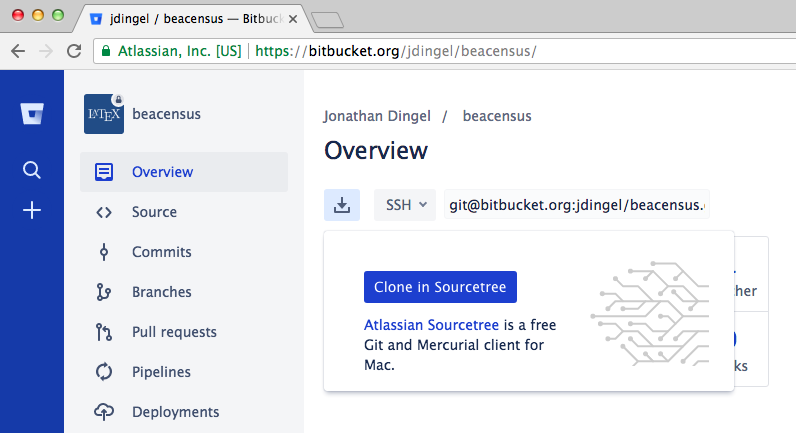
\includegraphics[width=.8\textwidth]{./figures/workflow/BitBucket_screeshot_cloneinsourcetree1.png}
\end{center}
Name the folder on your machine, and a copy of all the files in the remote repository will be cloned to your local repository.

It's also possible to clone remote repositories to which you have access simply by opening the SourceTree app and following \href{https://confluence.atlassian.com/get-started-with-sourcetree/clone-a-remote-repository-847359098.html}{these instructions}.

You'll want to set the username and email address in your \texttt{.gitconfig} file
to match the email address you're using on \href{http://www.github.com}{GitHub.com} or \href{http://www.bitbucket.org}{BitBucket.org}
so that commits are properly associated with your user account.

\subsubsection{Pull and push}

Two commands, \textbf{git pull} and \textbf{git push},
allow us to sync the local repo and remote repo.
You ``pull'' commits from the remote repo down to your local repo;
you ``push'' commits from your local repo to the cloud.

You must pull before you push.
You can pull after you commit, but if you commit and there are already new commits in the remote repo, you have to pull those commits and merge them with yours before you're allowed to push your commit to the remote repo.\footnote{
	Git Basics \href{https://git-scm.com/book/en/v2/Git-Basics-Working-with-Remotes\#_pushing_remotes}{2.5} on \texttt{git push}: ``This command works only if you cloned from a server to which you have write access and if nobody has pushed in the meantime. If you and someone else clone at the same time and they push upstream and then you push upstream, your push will rightly be rejected. You'll have to fetch their work first and incorporate it into yours before you'll be allowed to push.''
}
It's best to pull before you commit, just to reduce the number of ``merge'' commits that appear in the project history.
But if you're working on the same file as a collaborator, merges are unavoidable.
Git isn't Dropbox: if you ignore a project for a couple weeks, nothing will sync automatically.
But there's no reason to pull regularly if you're not looking at a project.
Pull when you sit down to resume work.

Relative to the single-machine process of doing a chunk of work and committing it,
the collaborative process involves only one extra step:
push after you commit.
\begin{lstlisting}[language=bash]
cd /path/to/repo
git pull
# make some changes to a file named "test.txt"
git add test.txt
git commit -m "edited test.txt"
git push
\end{lstlisting}


\subsubsection{Branching and merging}
A branch is series of commits that can be distinguished from another collection of commits.
Branches allow you to make commits without immediately having that code be imposed on the master project.
The merit of branching is most obvious when you're doing web development in which your service is always ``live''.
If the ``master'' branch is your live website, you don't want version 0.1 of a new feature to immediately go live.
In that case, the master branch must be immaculate, and branches are where development happens.
Once new features (or rewrites of old features) are tested and proven, they're merged into the master branch.

Research doesn't quite follow this model.
It's unlikely that there's a ``live'' version.
On the other hand, we often rewrite code when something is slow or inefficient.
For large chunks of work (or for rewrites that should deliver identical output), it makes sense to work on your own branch so that others' downstream work isn't altered until you're ready to merge into the master branch.
We create a new branch whenever we create a new task or substantially rewrite an old task.
See Section~\ref{code_review_process} for more about the role of branching within our code writing and reviewing processes.

The \texttt{git branch} command lets you create, list, rename, and delete branches.
It is tightly integrated with the \texttt{git checkout} and \texttt{git merge} commands.
\begin{lstlisting}[language=bash]
git branch
# List all of the branches in your repository.

git branch <branch>
# Create a new branch called <branch>. This does not check out the new branch.

git branch -d <branch>
# Delete the specified branch. This is a ``safe'' operation in that Git prevents
# you from deleting the branch if it has unmerged changes.

git branch -D <branch>
# Force delete the specified branch, even if it has unmerged changes. This is
# the command to use if you want to permanently throw away all of the commits
# associated with a particular line of development.

git branch -m <branch>
# Rename the current branch to <branch>.

git checkout <existing-branch>
# Check out the specified branch, which should have already been created with
# git branch. This makes <existing-branch> the current branch, and updates the
# working directory to match.

git checkout -b <new-branch>
# Create and check out <new-branch>. The -b option is a convenience flag that
# tells Git to run git branch <new-branch> before running git checkout
# <new-branch>. git checkout -b <new-branch> <existing-branch>

git merge <branch>
# Merge the specified branch into the current branch. Git will determine the
# merge algorithm automatically (discussed below).

git merge --no-ff <branch>
# Merge the specified branch into the current branch, but always generate a
# merge commit (even if it was a fast-forward merge).
\end{lstlisting}

In some cases, you might forget to pull the latest commit before making a new one.
As a result, you might be unable to push your commit due to a \href{https://happygitwithr.com/push-rejected.html}{conflict} with the latest commit on a repository.
To find a solution, read \href{https://happygitwithr.com/pull-tricky.html}{Chapter 28 Pull, but you have local work}.
